\documentclass[a4paper, 12pt, oneside]{article}
\usepackage{etex}
\reserveinserts{28}

\usepackage{comment}
\usepackage{lipsum} % for some dummy text

%%% Работа с русским языком
\usepackage{cmap}					% поиск в PDF
\usepackage{mathtext} 				% русские буквы в фомулах
\usepackage[T1,T2A]{fontenc}
\usepackage[utf8]{inputenc}			% кодировка исходного текста
\usepackage[english,russian]{babel}	% локализация и переносы

%%% Дополнительная работа с математикой
\usepackage{amsmath,amsfonts,amssymb,amsthm}
\usepackage{mathtools}
\usepackage{icomma} % "Умная" запятая: $0,2$ --- число, $0, 2$ --- перечисление

%% Номера формул
\mathtoolsset{showonlyrefs=true} % Показывать номера только у тех формул, на которые есть \eqref{} в тексте.

%% Шрифты
\usepackage{euscript}	 % Шрифт Евклид
\usepackage{mathrsfs}    % Красивый матшрифт
\usepackage{gensymb}     % Основные символы (degree sign)
\usepackage{csquotes}

% Таблицы
\usepackage{tabularx}
\usepackage{tabulary}

% Гиперссылки
\usepackage{hyperref}
\usepackage[usenames,dvipsnames,svgnames,table,rgb]{xcolor}
\hypersetup{				% Гиперссылки
	unicode=true,           % русские буквы в раздела PDF
	pdftitle={Конспект по курсу Наноматериалы},   % Заголовок
	pdfauthor={Л.Б.Матюшкин, \\ асс. каф. микро- и наноэлектроники СПбГЭТУ <<ЛЭТИ>>},      % Автор
	pdfsubject={Тема},      % Тема
	pdfcreator={Создатель}, % Создатель
	pdfproducer={Производитель}, % Производитель
	pdfkeywords={keyword1} {key2} {key3}, % Ключевые слова
	colorlinks=true,       	% false: ссылки в рамках; true: цветные ссылки
	linkcolor=blue,          % внутренние ссылки
	citecolor=blue,         % на библиографию
	filecolor=magenta,      % на файлы
	urlcolor=blue           % на URL
}

%%% Список условных обозначений
\usepackage{glossaries}
\makeglossary    % Закомментируйте, если перечень не нужен

%%% Изображения
\usepackage{graphicx, color}
\graphicspath{{../images/}}

%%%Работа с цветом текста
\usepackage{color}
\newcommand{\hl}[1]{\colorbox{yellow}{#1}} % подсветка желтым


% Список условных обозначений
\usepackage{nomencl}
\makenomenclature
\newcommand*{\nom}[2]{#1\nomenclature{#1}{#2}}
\makeatletter
\patchcmd{\thenomenclature}{\section*}{\section}{}{}
\makeatother
\renewcommand{\nomname}{Перечень условных обозначений}

%%% Предметный указатель
\usepackage{makeidx}  % Составление предметного указателя
\makeindex
%\usepackage{showidx} % Показать части предметного указателя на правом поле

\frenchspacing

% Библиотека для добавления текста к рисунку
\usepackage[percent]{overpic}
\usepackage{nicefrac}

\clubpenalty = 10000

%%% Простая графика
\usepackage{tikz}
\usetikzlibrary{arrows, mindmap, trees, shadows, shapes, calc, fadings, positioning, decorations.pathreplacing, intersections}
\tikzset{>=latex}

%% Свои команды
\DeclareMathOperator{\sgn}{\mathop{sgn}}

\newcommand*{\hm}[1]{#1\nobreak\discretionary{}
	{\hbox{$\mathsurround=0pt #1$}}{}}

%% Оформление химических формул
\newcommand*\chem[1]{\ensuremath{\mathrm{#1}}}

\renewcommand{\ge}{\geqslant}
\renewcommand{\le}{\leqslant}

%%%Подключение библиографии
%\usepackage[backend=biber, natbib=true, style=numeric-comp, sorting=none]{biblatex}
%\addbibresource{Bibs/Matyushkin.bib}

\title{Фрактальные фотонные кристаллы}
\author{Л.\:Б.\:Матюшкин \\  \href{mailto:leva.matyushkin@gmail.com}{leva.matyushkin@gmail.com}\\
	СПбГЭТУ <<ЛЭТИ>>}
\date{\today}

% Индексирование для создания предметного указателя
\makeindex
%\includeonly{0D/metal_nanoparticles}

\begin{document}

\maketitle
	Рассмотрены оптические свойства многослойных структур на основе диоксидов кремния и титана, толщины слоев которых соотносятся между собой как элементы канторова множества. Исследовано влияние правил разбиения пространства структуры на спектры пропускания.

\section*{Введение}
Современные технологии синтеза тонких пленок, такие как метод атомно-слоевого осаждения (ALD), позволяют создавать структуры с прецизионной точностью до единиц и даже десятых долей нм. При этом толщины структур, технологически задаваемые количеством циклов осаждения, могут изменяться в широком интервале размеров. Это создает предпосылки для создания структур с фрактальными отношениями толщин слоев, в частности оптических структур.

Структуру классического фотонного кристалла можно представить в виде чередующихся слоев материалов с низким и высоким значением показателя преломления --- обозначим их $S$ (\emph{silica}) и $T$ (\emph{titania}).

\section{Модель структуры}
Моделирование проводилось с учетом известных законов дисперсии показателей преломления наиболее популярной пары материалов --- оксида кремния \chem{SiO_2} и оксида и титана \chem{TiO_2}, взятых из базы данных http://refractiveindex.info/. Соответствюущие зависимости имеют вид:
	
$$n_{SiO_2}= \sqrt{1 + \frac{0.6961663\lambda^2}{\lambda^2-0.0684043^2}+\frac{0.4079426\lambda^2}{\lambda^2-0.1162414^2}+\frac{0.8974794\lambda^2}{\lambda^2-9.896161^2}}$$

$$n_{TiO_2}= \sqrt{5.913+\frac{0.2441}{\lambda^2-0.0803}}$$

При моделировании также учитывалась среда, в которой находится структура (в наиболее распространенном случае воздух):

$$n_{air}= 1+\frac{0.05792105}{238.0185-\lambda^{-2}}+\frac{0.00167917}{57.362-\lambda^{-2}}$$

Так как приведенные зависимости были получены для различных интервалов длин волн, мы рассматривали общую часть этих интервалов --- 0,4--1,5 мкм. Для удобства отображения спектров мы использовали принятые в спектроскопии координаты волнового числа $k = 1/\lambda$.

\section{Влияние правила замены}



С позиций фрактальной геометрии структуру классического фотонного кристалла $STSTSTS\dots$ можно рассматривать как частный случай принципа самоподобия, когда при замене $S \rightarrow STS$ не происходит скейлинга элемента $T$. Представим, что в структуре чередующихся слоев произошел скейлинг, соответствующий замене $T \rightarrow TTT$:  

\begin{multline}
S \rightarrow STS \rightarrow STSTTTSTS \rightarrow \\
\rightarrow STSTTTSTSTTTTTTTTTSTSTTTSTS \rightarrow \dots 
\end{multline}

\begin{figure}[h!]
	\centering
	\includegraphics[width=1.0\textwidth]{structureSTS0}
	\includegraphics[width=1.0\textwidth]{structureSTS1}
	\includegraphics[width=1.0\textwidth]{structureSTS2}
	\includegraphics[width=1.0\textwidth]{structureSTS3}
	\includegraphics[width=1.0\textwidth]{structureSTS4}
	\includegraphics[width=1.0\textwidth]{structureSTS5}
	\caption{Структура фрактального ФК на различных итерациях $C_i: S \rightarrow STS, i = 0 \dots 5$}
	\label{fig:structureSTS}
\end{figure}

\begin{figure}[h!]
	\centering
	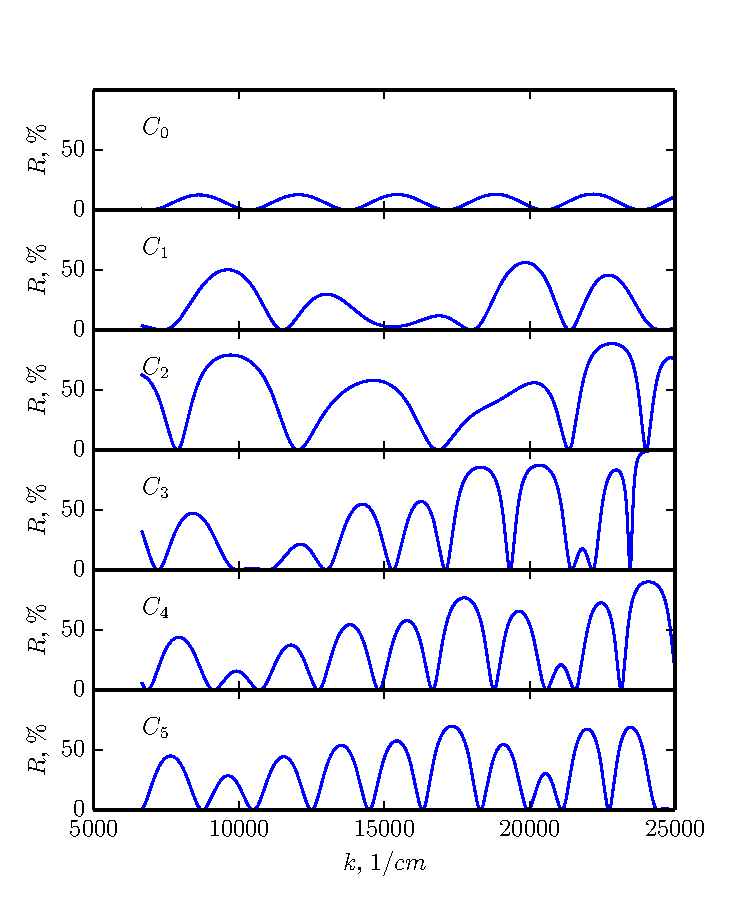
\includegraphics{STS}
	\caption{Cпектры отражения фрактального ФК $C_i: S \rightarrow STS$}
	\label{fig:spectraSTS}
\end{figure}

Считая, что между слоями повторяющихся материалов нет границы раздела, можно сопоставить каждому такому множеству однотипных символов пропорциональные толщины материалов, ставя в соответствие общей толщине структуры длину строки символов (Рис. \ref{fig:structureSTS}). При одной и той же толщине структуры повторение описанной процедуры приводит к быстрому уменьшению толщины самых тонких слоев структуры. В описанном случае толщина самого малого элемента уменьшается как $h/3^n$, где $h$ --- толщина структуры в целом, $n$ --- номер итерации.

Стоит заметить, что количество слоев с учетом описанного правила повторяющихся элементов нарастает медленнее --- как $2^{n+1}-1$, что важно с практической точки зрения получения таких структур.

В большинстве случаев мы исходили из возможности получения слоев с точностью 1 нм и общей толщиной структуры 1 мкм. Для таких ограничений максимальное количество имеющих физический смысл итераций составляет 4--5, что соответствует чередованию $\sim$30--60 слоев. Поэтому в расчете не рассматривается большее количество итераций.

\begin{figure}[h!]
	\centering
	\includegraphics[width=1.0\textwidth]{structureTST0}
	\includegraphics[width=1.0\textwidth]{structureTST1}
	\includegraphics[width=1.0\textwidth]{structureTST2}
	\includegraphics[width=1.0\textwidth]{structureTST3}
	\includegraphics[width=1.0\textwidth]{structureTST4}
	\includegraphics[width=1.0\textwidth]{structureTST5}
	\caption{Структура фрактального ФК на различных итерациях $C_i: T \rightarrow TST, i = 0 \dots 5$}
	\label{fig:structureTST}
\end{figure}

\begin{figure}[h!]
	\centering
	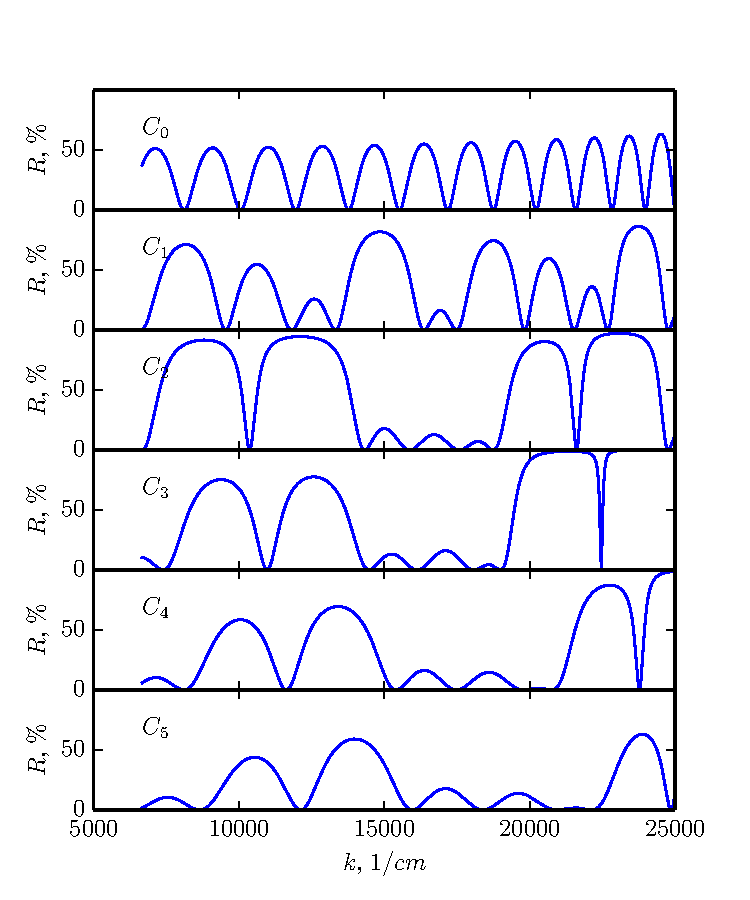
\includegraphics{TST}
	\caption{Cпектры отражения фрактального ФК $C_i: T \rightarrow TST$}
	\label{fig:spectraTST}
\end{figure}

\subsection{Сравнение с классическим фотонным кристаллом}

Можно заметить, что структура $C_1$ соответствует обычной очередности в фотонном кристалле из трех слоев (? как назвать), а структура $C_2$ повторяет структуру классического фотонного кристалла из 9 слоев за исключением средней части, и т.\:д. В рамках фрактальной геометрии можно рассматривать структуру фотонного кристалла как использование правила, когда одновременно выполняются замены:
$$C_i: S \rightarrow STS, T \rightarrow TST.$$ Соответствующие структуры представлены на Рис. \ref{fig:structurePC}.

\begin{figure}[h!]
	\centering
	\includegraphics[width=1.0\textwidth]{structurePC0}
	\includegraphics[width=1.0\textwidth]{structurePC1}
	\includegraphics[width=1.0\textwidth]{structurePC2}
	\includegraphics[width=1.0\textwidth]{structurePC3}
	\includegraphics[width=1.0\textwidth]{structurePC4}
	\includegraphics[width=1.0\textwidth]{structurePC5}
	\caption{Структура классического ФК на различных итерациях $C_i: S \rightarrow STS, T \rightarrow TST$}
	\label{fig:structurePC}
\end{figure}


\begin{figure}[h!]
	\centering
	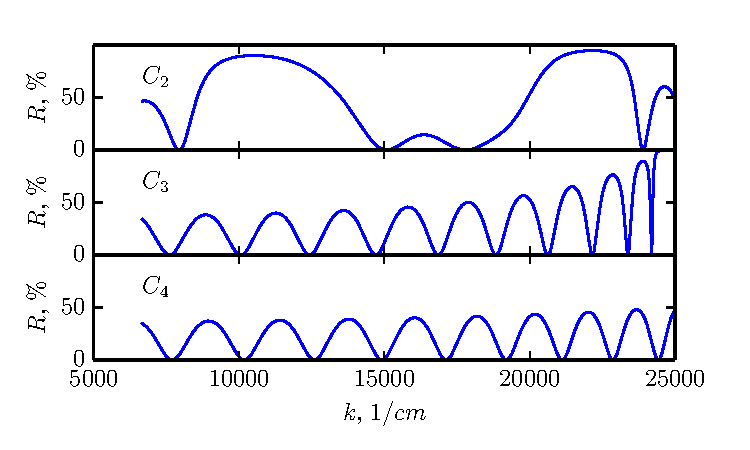
\includegraphics{PC}
	\caption{Cпектры отражения классического ФК $C_i: S \rightarrow STS, T \rightarrow TST$}
	\label{fig:spectraPC}
\end{figure}

\subsection{Изменение центральной вставки}

В случае изменения исходного правила $STS \rightarrow STTS$ (то есть при увеличении внутренней вставки), происходит существенное изменение спектра. В этом случае слои оптически менее плотного материала удаляются друг от друга за счет фрактального повторения более широкой вставки оптически плотного материала:

$$S \rightarrow STTS \rightarrow STTSTTTTTTTTSTTS \rightarrow \dots$$

Количество чередующихся слоев остается по-прежнему $2^{n+1}-1$.

\begin{figure}[h!]
	\centering
	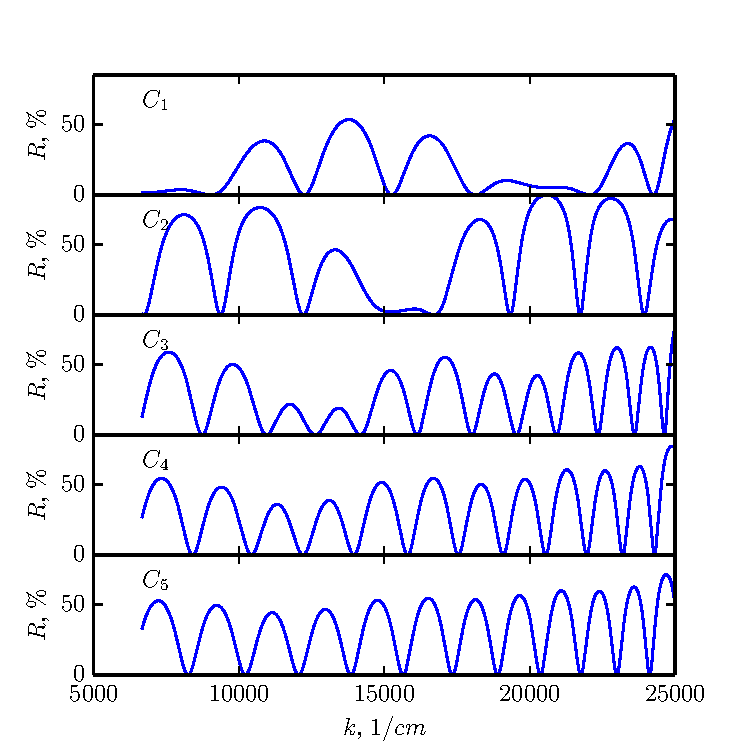
\includegraphics{STTS}
	\caption{Cпектры отражения фрактального ФК при изменении центральной вставки $C_i: S \rightarrow STTS$}
	\label{fig:spectraSTTS}
\end{figure}

На Рис. \ref{fig:spectraTSST} можно видеть, что структура $C2$ для $TSST$ может использоваться как структура фильтра.

\begin{figure}[h!]
	\centering
	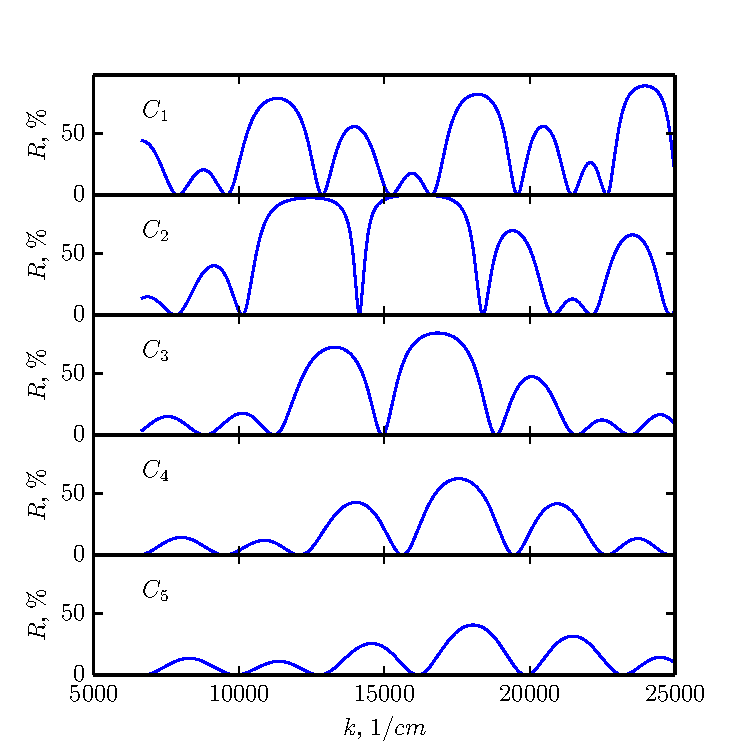
\includegraphics{TSST}
	\caption{Cпектры отражения фрактального ФК при изменении центральной вставки $C_i: T \rightarrow TSST$}
	\label{fig:spectraTSST}
\end{figure}

\subsection{Правило попеременной замены}

\section{Влияние размера структуры}

\subsection{Соотнесение}

\subsection{Усиление эффекта повтором}

\subsection{Половинчатые структуры}

Рассмотрим как повлияет на спектр использование половины исходной структуры.

\section{Заключение}
	
\end{document}